%
% Chapter 11
%

\chapter{Statistical Methods}
The \tth signal process, as well as the background, is inherently subject to statistical fluctuations due to quantum mechanics.
Additional randomness is introduced in the measurement process. This inherent randomness means that simply counting the number of predicted
signal and background events, and counting the number of events observed from data and comparing the two numbers is not necessarily enough to infer the presence or
lack thereof of the \tth signal process. Instead, the degree to which the
number of events in the signal and background predictions agree, given their uncertainties, with the number of events observed in data, must be quantified.
Furthermore we must quantify the probability that the numbers we observe are representative of nature at large, and not a statistical fluctuation driven by randomness. 
We use the likelihood function as the basis for estimating the signal strength parameter via the maximum likelihood technique, and also for composing our test statistic when
calculating upper limits  on the signal strength parameter via the CLs method. 


\section{Maximum Likelihood Fit}
The likelihood function is defined as the probability density of the number of observed events, $N$, given the predicted number of signal plus background events, $\mus + b$,
where $\mu$ is the signal strength parameter we wish to estimate. $\mu$ is more generally referred to as the parameter of interest, since it is free to float to the value
which best fits the observation. The signal strength parameter is assumed to be a modifier on the cross section of the \tth signal process, and does not depend on repeated
observations or bins. The simplified likelihood, ignoring nuisance parameters for now, is written as a Poisson probability under the freqentist approach as:

\begin{equation}
\label{eqn:likelihood1}
\mathcal{L}(data|\mu) = P(N|\mu s+b) = \frac{(\mu s+b)^{N}e^{-(\mu s+b)}}{N!}
\end{equation}

\noindent The above expression holds for a single bin of events, however this analysis is performed in each subcategory of the signal
region for each bin of the final BDT discriminant. The likelihood for this analysis must be calcualted separately for each bin of each signal region category $i$, and
the corresponding number of observed events in data $n_{i}$, and predictions of signal and background, $s_{i}, b_{i}$ respectively:

\begin{equation}
\label{eqn:likelihood2}
\mathcal{L}(data|\mu) = \prod_{i=1} \frac{(\mu s_{i}+b_{i})^{n_{i}}e^{-(\mu s_{i}+b_{i})}}{n_{i}!}
\end{equation}

\noindent Now the uncertainties associated with the signal and background predictions must be accounted for in the form of nuisance parameters. The expected signal
and background yields are re-written $s \rightarrow s(\theta)$ and $b \rightarrow b(\theta)$ to depend on the set of nuisances $\theta$. The expected value of the nuisances
is $\tilde{\theta}$. The nuisances are parametrized as a PDF $P(\theta|\tilde{\theta})$. With Bayes' theorem, this PDF becomes:

\begin{equation}
\label{eqn:nuisance}
P(\theta|\tilde{\theta}) ~ P(\tilde{\theta}|\theta) \cdot \pi(\theta)
\end{equation}

In this context, $P(\theta|\tilde{\theta})$ is the posterior probability, or the degree to which we believe the true value of $\theta$ given our estimate $\tilde{\theta}$.
$P(\tilde{\theta}|\theta)$ is interpreted as the probability of obtaining the value $\tilde{\theta}$ when the true value is $\theta$. $\pi(\theta)$ is the prior.
In this analysis, the prior is a gaussian distribution for shape systematics, and a log-normal distribution for rate systematics. For gaussian and log-normal distributions,
the prior $\pi(\theta)$ does not vary significantly with $\theta$. We can solve Equation~\ref{eqn:nuisance} for $P(\tilde{\theta}|\theta)$, which constrains the nuisances
and the likelihood can be modified properly:

\begin{equation}
\label{eqn:likelihood3}
\mathcal{L}(data|\mu,\theta) = \prod_{i=1} \frac{(\mu s_{i}(\theta)+b_{i}(\theta))^{n_{i}}e^{-(\mu s_{i}(\theta)+b_{i}(\theta))}}{n_{i}!} \cdot P(\tilde{\theta}|\theta)
\end{equation}

\noindent The estimated value for $\mu$ is obtained from finding the values of $\mu$ and $\theta$ which maximize the likelihood, denoted as $\hat{\mu}$ and $\hat{\theta}$.
This technique is called the maximum likelihood estimation (MLE)~\cite{lista}.
In practice, we first take the negative log of the likelihood (NLL), and then find the minimum, since it simplifies
the procedure by turning the product in Equation~\ref{eqn:likelihood3} into a sum. $\hat{\mu}$ is referred to as the ``best-fit'' $\mu$, because it is the value which best fits the data.
This maximum likelihood procedure is also referred to generally as the ``fit''. 

\section{Upper Limits: CLs Method}
When an analysis lacks the sensitivity to detect a signal from background, setting uppper limits on the possible values of $\mu$ is useful. In setting upper
limits, $\mu$ is constrained as phase space is excluded. This strategy was used by the Higgs analyses at LEP and the Tevatron, and is the primary figure of merit
for an analysis with little sensitivity. The \tth analysis presented here does not fall into this category, although previous iterations lacked the sensitivity
to detect \tth in data. While this analysis does have sensitivity to \tth, upper limits are still set using the CLs method, also known as the
Modified Frequentist approach, which builds on the likelihood described in the previous section. 

Starting from the likelihood in Equation~\ref{eqn:likelihood3}, we construct a test statistic, $q_{\mu}$, based on the profile likelihood ratio\footnote{The ``profile'' in profile
likelihood ratio is due to the fact that the nusiance parameter values are constrained from a fit to data.}~\cite{AsymptoticLimits},
defined as:

\begin{equation}
\label{eqn:test_stat}
\tilde{q}_{\mu} = -ln \frac{\mathcal{L}(data|\mu,\hat{\theta_{\mu}})}{\mathcal{L}(data|\hat{\mu},\hat{\theta})},~~~~~0 \leq \hat{\mu} \leq{\mu}
\end{equation}

\noindent Where $\hat{\theta_{\mu}}$ is the value of the nusiances corresponding to $\mu$. $\mathcal{L}(data|\mu,\hat{\theta_{\mu}})$ is the maximized where $\mu$
is fixed to some value and $\hat{\theta_{\mu}}$ floats freely. The denominator, $\mathcal{L}(data|\hat{\mu},\hat{\theta})$, is the maximum likelihood obtained
previously where both parameters float. The lower bound $0 \leq \hat{\mu}$ ensures the signal is positive. The upper bound $\hat{\mu} \leq \mu$ imposes a one-sided
confidence interval, which practically means that upward fluctuations of data $\hat{\mu} > \mu$, where the hypothesis is $\mu$, cannot be considered as evidence
against the hypothesis.  

With the definition of the test statistic, we calculate $\tilde{q}_{\mu}^{obs}$, the observed test statistic value in data, by evaluating it for many different
values of $\mu$. Now the values for the nuisance parameters observed in data, $\hat{\theta_{0}^{obs}}$, $\hat{\theta_{\mu}^{obs}}$ are obtained from maximizing
the likelihoods under the background only ($\mu=0$), and signal plus background hypotheses respectively. Next, two test statistic PDFs
$f(\tilde{q}_{\mu}|\mu,\hat{\theta_{\mu}^{obs}})$, and $f(\tilde{q}_{\mu}|0,\hat{\theta_{0}^{obs}})$ are constructed from psuedo-data
generated with MC toys, obtained from random sampling of nusiance parameter values from the fit to data at fixed $\mu$.  Next we calculate a p-value $p_{\mu}$, $p_{b}$
for the signal plug background and background only hypotheses. The p-value $p_{\mu}$ represents the probability that the observed data is incompatible with the
signal plus background hypothesis, with signal strength $\mu$. As $p_{\mu}$ decreases, the more confident we are that the value of $\mu$ being evaluated is the
upper limit on the signal strength. The p-value $p_{b}$ is the probability for compatibility with the background only hypothesis. As $p_{b}$ decreases, the probability
of a signal in the data increases. It is more convenient to work with $1-p_{b}$, since this value is the probability of incompatibility with the background only hypothesis,
just as $p_{s}$ is a probability of incompatibility with the signal plus background hypothesis:

\begin{equation}
\label{eqn:pvalues1}
p_{\mu} = P(\tilde{q}_{\mu} \geq \tilde{q}_{\mu}^{obs}|signal+background) = \int_{\tilde{q}_{\mu}^{obs}}^{\infty} f(\tilde{q}_{\mu}|\mu,\hat{\theta_{\mu}^{obs}}) d\tilde{q}_{\mu}
\end{equation}

\begin{equation}
\label{eqn:pvalues2}
1- p_{b} = P(\tilde{q}_{\mu} \geq \tilde{q}_{\mu}^{obs}|background only) = \int_{\tilde{q}_{0}^{obs}}^{\infty} f(\tilde{q}_{\mu}|0,\hat{\theta_{0}^{obs}}) d\tilde{q}_{\mu}
\end{equation}

\noindent We define confidence levels (CL) for each hypothesis, with $CL_{s+b} = p_{\mu}$, and $CL_{b} = 1-p_{b}$, with $CL_{s}$ being the ratio of the two:

\begin{equation}
\label{eqn:cls}
CL_{s}(\mu) = \frac{CL_{s+b}}{CL_{b}} = \frac{p_{\mu}}{1-p_{b}}
\end{equation}

\noindent Interpreting Equation~\ref{eqn:cls}, we can say that as the probability for incompatibility with the background only hypothesis increases, and/or as the probability
for incompatibility with the signal plus background hypothesis decreases, $CL_{s}(\mu)$ will decrease, and we become more confident that the observed data is more consistent with
the signal plus background hypothesis than the background only hypothesis. The 95$\%$ CL upper limit on $\mu$ is obtained by testing different values of decreasing $\mu$ and
calculating $CL_{s}(\mu)$, the upper limit is the value of $\mu$ for which $CL_{s}(\mu) = 0.05$. In general we say that for some $\mu$ corresponding to $CL_{s}(\mu) \leq \alpha$
the signal is excluded at the $1-\alpha$ CL. 




%For the purpose of setting upper limits on the value of $\mu$, we first define condfidence level (CL) integrals to specify a range of values for $\mu$ for which we are quantifiably
%certain contains the true value. The denominator, $\mathcal{L}(data|\hat{\mu},\theta)$, is the maximum likelihood obtained from the maximization in Equation~\ref{eqn:likelihood3},
%where both parameters float. 



  
%With the statistics available in this analysis, the best-fit $\mu$ and the corresponding significance are the primary metrics by which the analysis sensitivity is determined. 


%% given a set of experimental observables, evaluated at the values of those observables ($x_{1},...,x_{n}$)
%% that correspond to the data sample, for given values of unknown (nuisance) parameters ($\theta_{1},...,\theta_{m}$). The experimental observables consist of $n$ random
%% variables and the likelihood depends on the set of $m$ unknown parameters. The likelihood is expressed as:

%% The likelihood function is defined as the probability density, given a set of (experimental) observables, evaluated at the values of those observables ($x_{1},...,x_{n}$)
%% that correspond to the data sample, for given values of unknown (nuisance) parameters ($\theta_{1},...,\theta_{m}$). The experimental observables consist of $n$ random
%% variables and the likelihood depends on the set of $m$ unknown parameters. The likelihood is expressed as:

%% \begin{equation}
%% \label{eqn:likelihood1}
%% L(x_{1},...,x_{n}|\theta_{1},...,\theta_{m}) = f(x_{1},...,x_{n}|\theta_{1},...,\theta_{m})
%% \end{equation}

%% \noindent where $f$ is the joint PDF for a single event. With this, we define the \emph{maximum likelihood estimator} as the function that returns the values of parameters
%% $\theta_{1},...,\theta_{m}$ for which the likelihood function is maximum\footnote{It is assumed that there is a single, unique maximum value of the likelihood function}.
%% With $N$ repeated measurements ($N$ events), each with $n$ values of random variables ($x_{1},...,x_{n}$), with ($\theta_{1},...,\theta_{m}$) remaining constant across each
%% event, the full likelihood of the sample of $N$ un-correlated events is the product of the likelihoods for each event:

%% \begin{equation}
%% \label{eqn:likelihood2}
%% L(\textbf{x}|\overrightarrow{\theta}) = \prod_{i=1}^{N} f(x_{1}^{i},...,x_{n}^{i}|\theta_{1},...,\theta_{m})
%% \end{equation}

%% \noindent To simply the maximization procedure, the negative logarithm is taken to remove the product. Now the negative log likelihood in Equation~\ref{eqn:nll} is minimized.

%% \begin{equation}
%% \label{eqn:nll}
%% -ln L(\textbf{x}|\overrightarrow{\theta}) = -\sum_{i=1}^{N} ln f(x_{1}^{i},...,x_{n}^{i}|\theta_{1},...,\theta_{m})
%% \end{equation}

%% \noindent The above liklihood derivations do not assume that the number of events in the data sample is itself a random variable. In this analysis, the above likelihood definition must
%% be modified slightly since the number of events $N$ in the data sample \emph{is} a random variable, which depends on the set of unknown parameters ($\theta_{1},...,\theta_{m}$),
%% obeying some Poisson probability distribution $p(N|\theta_{1},...,\theta_{m})$\footnote{The PDF is a Poisson because the events are independent and occur within a fixed time interval}.
%% This is known as the extendend likelihood function written as:

%% \begin{equation}
%% \label{eqn:likelihood3}
%% L(N|\overrightarrow{\theta}) = \prod_{i=1}^{N} f(x_{1}^{i},...,x_{n}^{i}|\theta_{1},...,\theta_{m})
%% \end{equation}
 
%% \noindent Re-writing with the full Poisson probability this becomes:

%% \begin{equation}
%% \label{eqn:likelihood4}
%% L(N|\overrightarrow{\theta}) = \frac{e^{-\bar{\mu}($\theta_{1},...,\theta_{m}$)}\bar{\mu}($\theta_{1},...,\theta_{m}$)^{N}}{N!} \prod_{i=1}^{N} f(x_{1}^{i},...,x_{n}^{i}|\theta_{1},...,\theta_{m})
%% \end{equation}

%% \noindent Where $\bar{\mu}$ is the average of the Poisson and depends on the unknown parameters\footnote{Note that $\bar{\mu}$ is distinct from the signal strength measure, $\mu$}. In this analysis, the PDF 
%% is a linear combination of the signal and background, whose PDFs are denoted as $P_{s}$, $P_{b}$ with expected yields of $s$,$b$ respectively. The likelihood is now written as:

%% \begin{equation}
%% \label{eqn:likelihood4}
%% L(x_{i}|s,b,\theta) = \frac{e^{-(s+b)}(s+b)^{n}}{n!} \prod_{i=1}^{N} (f_{s}P_{s}(x_{i}|\theta) + f_{b}P_{b}(x_{i}|\theta))
%% \end{equation}

%% \noindent Where $f_{s} = \frac{s}{s+b}, f_{b} = \frac{b}{s+b}$ are the fractions of the expected signal and background events respectively.




\section{Limits}

\begin{table}[htbp]
\begin{center}
  \caption[Table of Final Limits]{95$\%$ CL upper limits on $\mu$ under the background-only hypothesis.}
    \begin{tabular}{c c} \hline
      Observed Limit & Expected Limit $\pm$1$\sigma$  \\ \hline 
      2.9 & 1.0$^{+0.5}_{-0.3}$  \\
      \hline
    \end{tabular}
    \label{tab:limits}
\end{center}
\end{table}

\section{Fit}

\begin{table}[htbp]
\begin{center}
  \caption[Table of best-fit signal strength]{}
    \begin{tabular}{c c c} \hline
      Observed $\mu$ fit $\pm$1$\sigma$ & Expected $\mu$ fit $\pm$1$\sigma$ & Observed(expected) significance & \\ \hline 
      1.7$^{+0.6}_{-0.5}$ & 1.0$^{+0.5}_{-0.5}$ & 3.3$\sigma$ (2.1$\sigma$)  \\
      \hline
    \end{tabular}
    \label{tab:mu}
\end{center}
\end{table}


\begin{table}[htbp]
  \begin{center}
    \caption[Signal region post-fit event yields by lepton flavor]{Expected (post-fit) yields for signal and background processes, and observed yields in data. Yields
      shown after a fit to data with all predictions constrained to SM expectation.}
    \begin{tabular}{l c c c} \hline
      & $\mu\mu$ & $ee$ & $e\mu$  \\ \hline 
      $t\bar{t}W$ & 45.4 $\pm$ 0.5 & 17.8 $\pm$ 0.3 & 64.3 $\pm$ 0.6 \\
      $t\bar{t}Z/\gamma^{*}$ & 16.8 $\pm$ 0.7 & 14.8 $\pm$ 0.8 & 41.7 $\pm$ 1.4 \\
      \hline
      WZ & 5.2 $\pm$ 0.7 & 1.6 $\pm$ 0.4 & 7.5 $\pm$ 0.8 \\
      Rare SM. bkg & 6.8 $\pm$ 0.3 & 3.5 $\pm$ 0.2 & 11.7 $\pm$ 0.4 \\
      WWss & 2.9 $\pm$ 0.2 & 1.4 $\pm$ 0.1 & 4.3 $\pm$ 0.2 \\
      \hline
      Conversions & 0.0 $\pm$ 0.0 & 3.4 $\pm$ 1.1 & 8.5 $\pm$ 1.3 \\
      Charge flip & 0.0 $\pm$ 0.0 & 172 $\pm$ 93 & 149 $\pm$ 82 \\
      Non-prompt leptons & 29.9 $\pm$ 1.2 & 17.3 $\pm$ 1.1 & 53.5 $\pm$ 1.8 \\
      \hline
      Total bkg & 107.3 $\pm$ 1.7 & 70.3 $\pm$ 1.8 & 208.0 $\pm$ 2.9 \\
      \hline
      $t\bar{t}H$ & 18.5 $\pm$ 0.2 & 7.4 $\pm$ 0.1 & 26.2 $\pm$ 0.2 \\
      \hline
      Data & 154 & 95 & 274 \\
      \hline
    \end{tabular}
    \label{tab:yields}
  \end{center}
\end{table}


\begin{figure}[htb]
        \centering 
        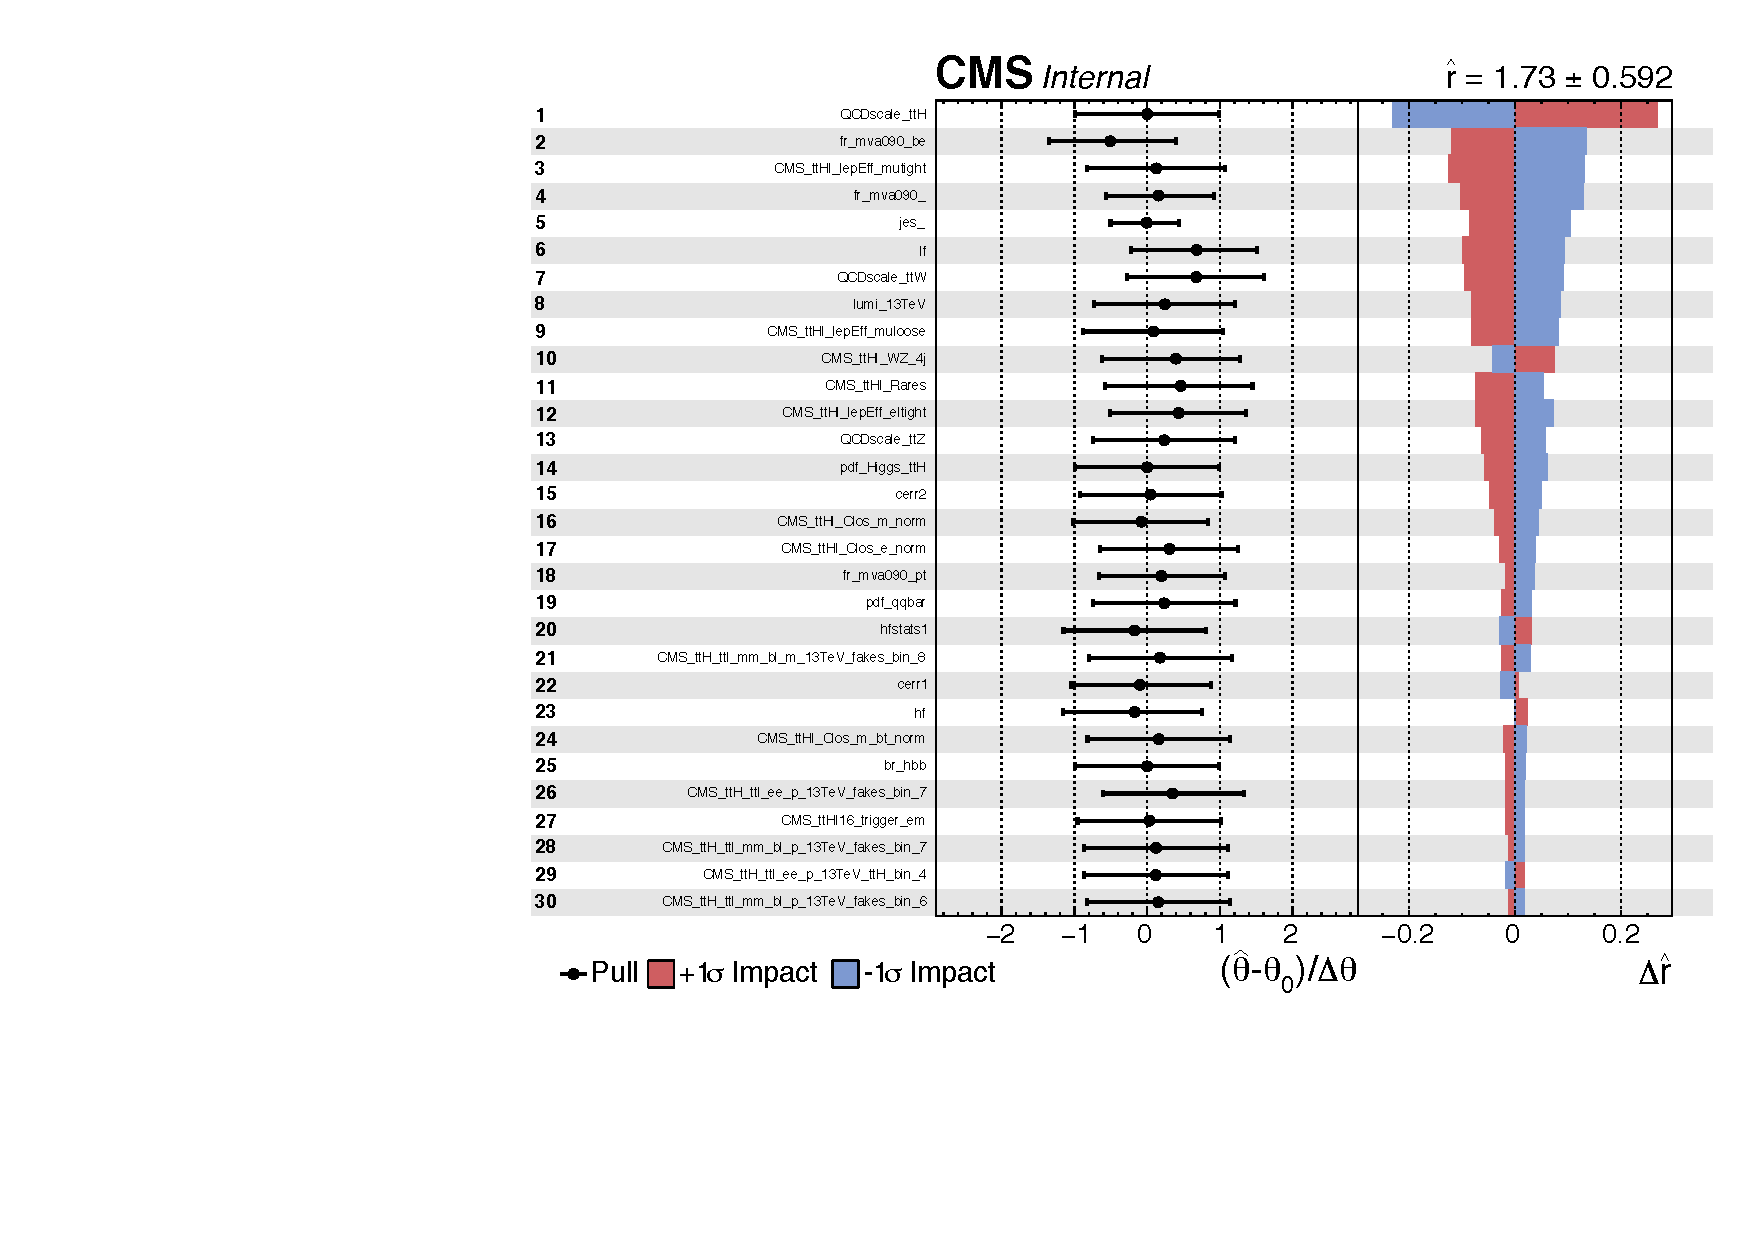
\includegraphics[width=0.95\textwidth]{ch11_figs/impacts_ttH_13TeV_top30.pdf}
        \caption[Nuisance parameter impacts]{The top nuisance parameters ranked by their impact on the fit. The pull of each nuisance (left) is the amount by which the fit moves that parameter from its
        initial value. The impact of each nuisance (right) is the change in best-fit $\mu$ divided by the uncertainty in $\mu$, obtained by moving each nuisance up (red) or down (blue) by 1$\sigma$.}
        \label{fig:impacts}
\end{figure}



\section{Conclusion}

%% \begin{figure}[hbtp]
%%  \begin{center}
%%    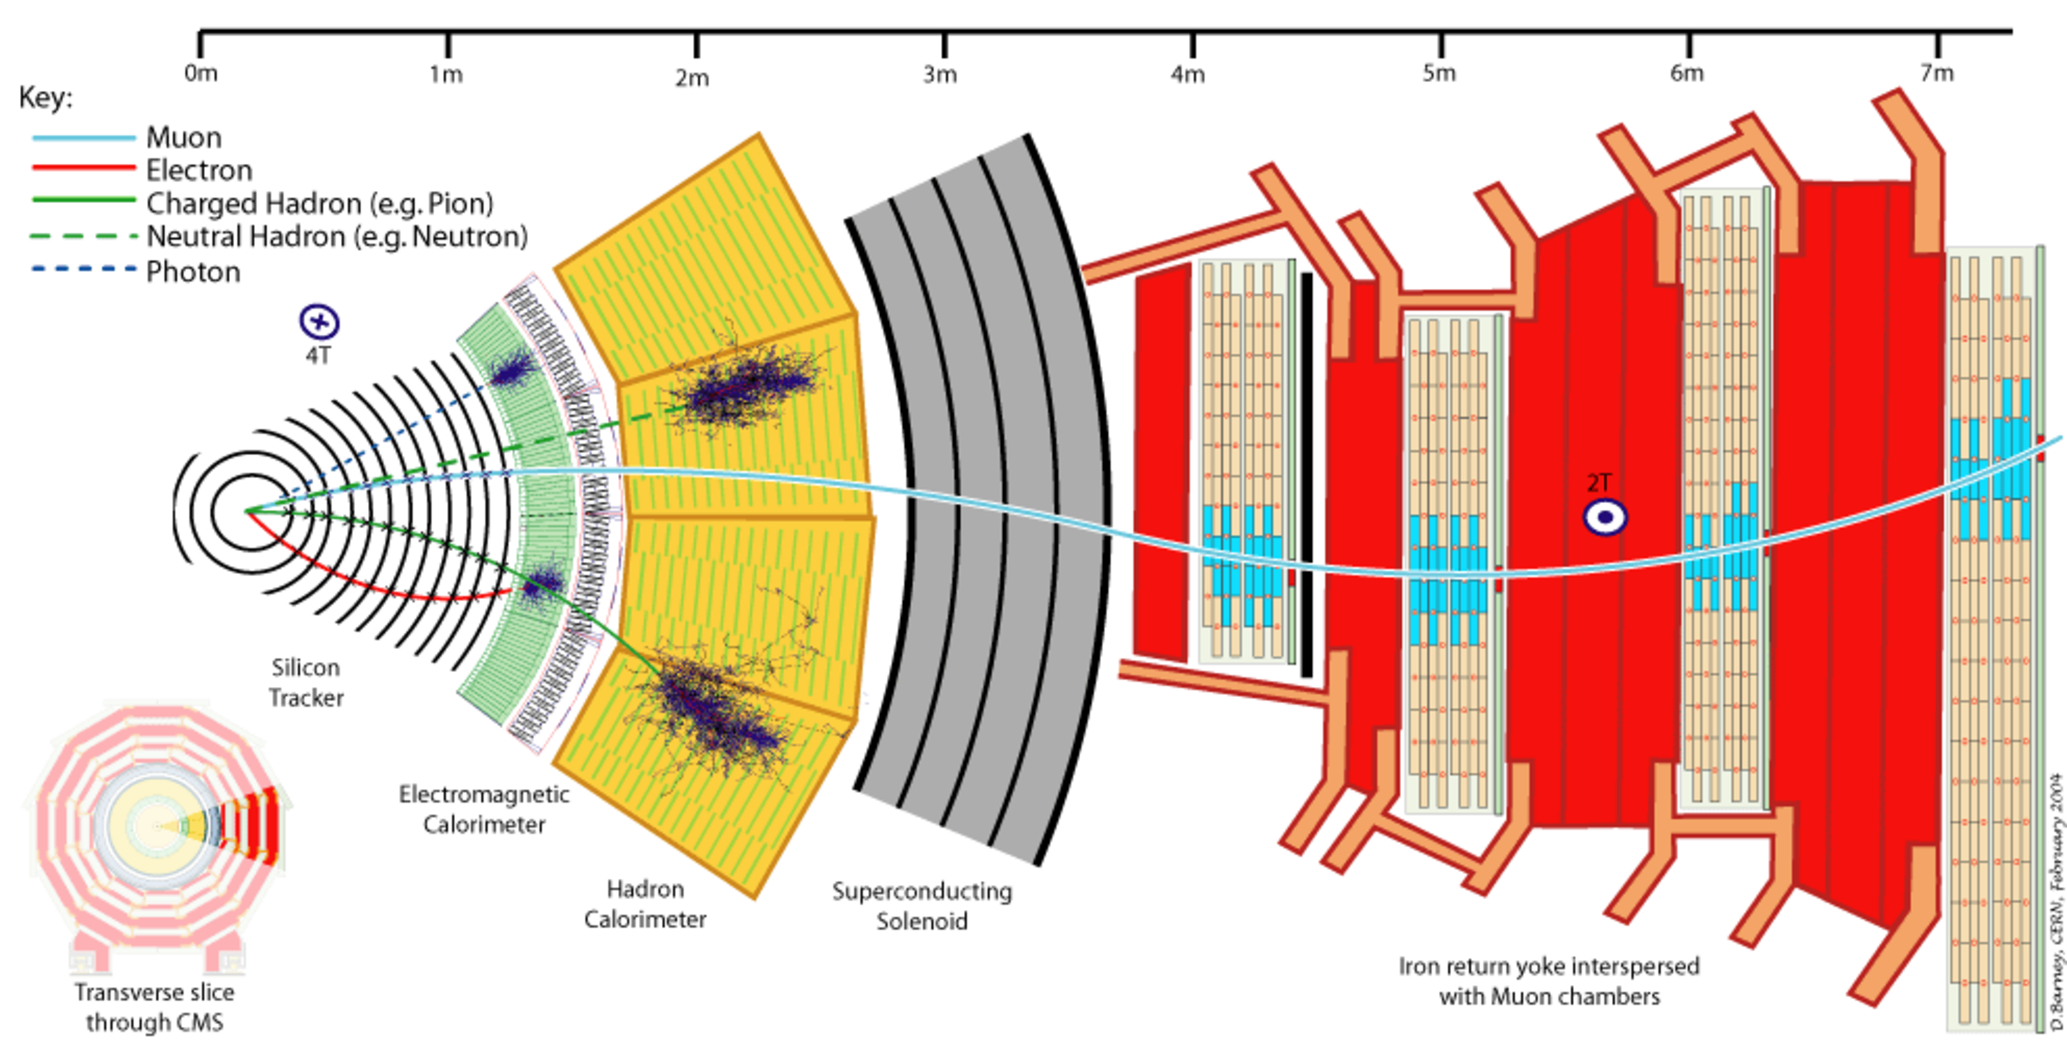
\includegraphics[width=0.8\textwidth]{ch4_figs/cms_particleflow.pdf}
%%    \caption{An overview of how CMS detects different types of particles. The slice of CMS in in the x-y plane.~\cite{NEED CITATION}.}
%%    \label{fig:cms_pflow}
%%  \end{center}
%% \end{figure}
